% ============================================================
%  CMP6200/DIG6200 --- Individual Undergraduate Project (FYP)
%  Project Final Report --- Smart Irrigation System (25-26)
%  Same template as the interim report (natbib Harvard, headers).
%  Compile: pdflatex && bibtex && pdflatex && pdflatex
%  Draw.io figures (separate files): docs/drawio/fig01_…fig17_….drawio
%  Export any file to PNG (same stem) to embed it; data plots 7–13 use results/figures/.
% ============================================================
\documentclass[12pt, a4paper]{article}

\usepackage[a4paper, margin=2.5cm]{geometry}
\usepackage{setspace}
\usepackage{parskip}
\usepackage{titlesec}
\usepackage{booktabs}
\usepackage{array}
\usepackage{tabularx}
\usepackage{longtable}
\usepackage{fancyhdr}
\usepackage{graphicx}
\usepackage{float}
\usepackage{enumitem}
\usepackage{xcolor}
\usepackage{tikz}
\usepackage{pgfgantt}
\usepackage{times}
\usepackage{microtype}
\usepackage{caption}
\usepackage[hidelinks]{hyperref}

\usepackage[authoryear, round]{natbib}
\bibliographystyle{plainnat}

\onehalfspacing
\setlength{\parindent}{0pt}
\setlength{\parskip}{6pt plus 2pt}

\titleformat{\section}{\large\bfseries}{\thesection}{1em}{}
\titleformat{\subsection}{\normalsize\bfseries}{\thesubsection}{1em}{}
\titlespacing*{\section}{0pt}{14pt}{6pt}
\titlespacing*{\subsection}{0pt}{10pt}{4pt}

\pagestyle{fancy}
\fancyhf{}
\rhead{\small CMP6200/DIG6200 --- Final Report}
\lhead{\small Smart Irrigation System}
\cfoot{\thepage}
\renewcommand{\headrulewidth}{0.4pt}

\hypersetup{
    colorlinks = true,
    linkcolor  = black,
    urlcolor   = black,
    citecolor  = black
}

\graphicspath{{../}{../../results/figures/}{../drawio/}}

% If you export a .drawio to PNG with the same file name, it is used here.
\newcommand{\drawiofigure}[4]{%
\begin{figure}[H]
\centering
\IfFileExists{../drawio/#1.png}{%
  \includegraphics[width=#2]{#1.png}}{%
  \fbox{\parbox{0.92\textwidth}{\centering\vspace{7mm}
  \texttt{docs/drawio/#1.drawio}\\[4pt]
  {\small diagrams.net: File $\rightarrow$ Export as $\rightarrow$ PNG}\\[1mm]
  {\small Save as \texttt{#1.png} next to the \texttt{.drawio} file.}
  \vspace{7mm}}}%
}
\caption{#3}
\label{#4}
\end{figure}%
}

\begin{document}

\pagenumbering{gobble}
\begin{titlepage}
    \centering
    \vspace*{2cm}
    {\Large\bfseries CMP6200/DIG6200\par}
    \vspace{0.5cm}
    {\large Individual Undergraduate Project (FYP)\par}
    \vspace{0.5cm}
    {\large\bfseries Project Final Report\par}
    \vspace{2cm}
    {\LARGE\bfseries Smart Irrigation System Using IoT and\\[6pt]
    Machine Learning for Sustainable Agriculture in Nepal\par}
    \vspace{2.5cm}
    \begin{tabular}{ll}
        \textbf{Student Name:} & Pramod Giri    \\[4pt]
        \textbf{Student ID:}   & 23189635       \\[4pt]
        \textbf{Course:}       & Final Year Project \\[4pt]
        \textbf{Supervisor:}   & Manoj Gautam   \\[4pt]
        \textbf{Date:}         & 20.09.2026     \\
    \end{tabular}
    \vfill
    {\small Main-text word count (abstract through Future Work): approximately 7{,}800, under the 10{,}000-word limit.}
\end{titlepage}

\pagenumbering{roman}

\begin{abstract}
Agriculture accounts for most of the world's freshwater withdrawals, so irrigation that follows soil and weather rather than a fixed calendar is a practical route to more sustainable food production \citep{almulla2022,liu2023}. In Nepal, smallholders still water largely by experience and routine, which wastes water in wet soil and under-waters crops during heat and high evaporative demand \citep{kunwar2024}. This report describes the design, construction, and evaluation of a closed-loop smart irrigation artefact for tomato: an ESP32 greenhouse node (temperature, humidity, soil moisture, optional pressure) posts live readings to a FastAPI service on a local computer; an XGBoost classifier returns a pump ON/OFF decision within seconds; a farmer dashboard states the action in plain language.

The machine-learning layer is trained on 3{,}000 Kathmandu field logs labelled with an FAO-56 tomato rule rather than the historical soil-only pump column. On a held-out 600-row split, XGBoost reaches F1~$0.993$ and ROC-AUC~$1.000$, and beats a 55\% soil-moisture cutoff (F1~$0.931$). Against an always-on calendar baseline the model irrigates on about 58\% of rows, a 42\% reduction in pump ON-time (above the 30\% water-saving target). Live deployment confirmed that the relay follows the API decision on every logged row and that air sensors are almost always readable. Two limitations remain material: the capacitive soil probe was not yet calibrated on the live bed (most live soil values sit at 0\%), and host-side gaps (computer asleep, Wi-Fi) keep calendar uptime well below the 95\% ambition. The contribution is a low-cost, locally hosted, tomato-specific decision loop that can run without a public cloud, and an honest account of where field sensing still needs work.
\end{abstract}

\tableofcontents
\newpage
\listoffigures
\listoftables
\newpage
\pagenumbering{arabic}

\section{Introduction and Context}
\label{sec:intro}

Agriculture is responsible for 70--80\% of global freshwater use. Improving irrigation is therefore a central part of any serious plan for sustainable food production \citep{almulla2022,liu2023}. Recent work on the Internet of Things (IoT), machine learning, and wireless sensor networks has shown that farms can decide when to water from measured soil and climate rather than from intuition or a fixed timetable \citep{singha2025,ikdid2021}. In many settings those traditional methods remain inefficient: they over-water, under-water, or both, and they leave preventable yield on the table \citep{naji2021,rajpoot2022}.

Nepal is a strong candidate for a locally adapted intervention. Around 60\% of the labour force works in agriculture, yet water supply is disrupted by monsoon seasonality, fragile infrastructure, and limited rural electrification \citep{kunwar2024,mool2001}. Hill and Terai systems already show conflict when canals run short \citep{kunwar2024} and inequity inside farmer-managed schemes \citep{upadhyay2015}. Tomato is a useful first crop for a student prototype: it is high-value, sensitive to both drought and waterlogging, and has a published FAO-56 management-allowed depletion near 0.40 \citep{allen1998}. A controller that is wrong for tomato is visibly wrong (cracked fruit, blossom-end rot, or a drowned root zone). Solutions designed for well-resourced experimental farms do not transfer unchanged. What is needed is a low-cost node that a smallholder can wire, a decision rule that understands tomato water stress rather than a generic soil switch, and software that does not depend on a paid public cloud.

This project therefore designed, built, and tested a smart irrigation prototype for tomato under Nepalese conditions. An ESP32 reads soil moisture, air temperature, humidity, and atmospheric pressure; a local FastAPI service stores each reading and runs a trained XGBoost model; the firmware drives a relay and pump from the returned \texttt{water\_needed} flag. The interim report posed the same problem and planned an LSTM on the ESP32 with MQTT to AWS. The artefact that was actually delivered changed that plan for reasons set out in Sections~\ref{sec:gap}--\ref{sec:methods}: the training logs have no timestamps, the pump needs an immediate ON/OFF decision rather than a 24-hour volume forecast, and a laptop on the same Wi-Fi is a more realistic host than AWS IoT Core for a student greenhouse trial.

The report is organised as follows. Section~\ref{sec:lit} reviews IoT irrigation, the Nepalese water context, and machine-learning decision methods, then names the gap this artefact fills. Section~\ref{sec:aims} states the aim, five SMART objectives, and the project boundary. Section~\ref{sec:design} describes methods and why they were chosen. Section~\ref{sec:artefact} specifies the six-layer design. Section~\ref{sec:implementation} records how the hardware, API, model, and dashboard were built and tested. Section~\ref{sec:evaluation} evaluates success against the literature and the objectives. Section~\ref{sec:conclusion} concludes, with limitations and future work. Feasibility, risks, and ethics are revised in Appendix~\ref{app:feasibility}.

\subsection{Problem Statement}
\label{sec:problem}

Nepalese smallholder farmers mainly set irrigation from experience and a fixed routine rather than from measured soil and weather \citep{kunwar2024}. Crops are therefore watered when the calendar says so, including when the root zone is already wet, and they are not watered extra when heat and vapour-pressure deficit raise tomato demand. This project addresses that gap with IoT sensing and a tomato-specific machine-learning decision, so that a pump on a monitored bed turns on only when the crop needs water.

\section{Review of Existing Knowledge}
\label{sec:lit}

The review is organised around four themes that sit behind the problem statement: sensor-based irrigation hardware, the Nepalese water and farm setting, machine-learning control, and whether farmers will actually use such tools.

\subsection{IoT-based smart irrigation}
\label{sec:iot}

\citet{singha2025} built an ESP32 system with soil moisture, humidity, and temperature sensors and reported a 12\% yield gain and a 58\% drop in water use versus traditional practice for red amaranth. \citet{naji2021} designed a low-cost wireless sensor network with Arduino and XBee for soil monitoring and irrigation control. \citet{rajpoot2022} compared sensor-based setups and found that they cut the labour of soil checking and supported plant growth; their agro-climate is close enough to Nepal's Terai for the hardware lessons to transfer. At community scale, \citet{ikdid2021} used a Penman--Monteith water-requirement model in a collaborative irrigation scheme, but the trial stayed in experimental conditions and did not ask whether smallholders would adopt it. Off-grid power remains a constraint: \citet{sohan2022} proposed a solar-powered, low-energy sensor network with battery backup, which this project treated as a reference architecture even though the student trial itself is mains-powered on a local computer.

A pattern across these IoT papers is that ``smart'' often means ``a moisture probe switches a pump''. That is already better than a weekly calendar, and it explains large water savings when the baseline is flood irrigation \citep{naji2021,singha2025}. It is not the same as crop-aware control. Soil moisture is necessary but not sufficient: two days at 50\% moisture are not equal if one is cool and humid and the other is hot with dry air. Papers that stop at a threshold therefore under-specify the decision the farmer actually needs. This project keeps the ESP32-class hardware from that literature and changes the decision layer.

\subsection{Nepal-specific agricultural context}
\label{sec:nepal}

International IoT papers have to be read against Nepal's hydrology and institutions. \citet{mool2001} mapped glaciers, glacial lakes, and outburst-flood risk, and noted that dry-season flows---the flows irrigation depends on---are sensitive to both monsoon timing and long-term ice loss. \citet{upadhyay2015} showed that farmer-managed schemes in hill districts struggle with unfair distribution and weak responses to crop stress in dry spells. \citet{kunwar2024} documents irrigation conflict where supply is unreliable. Together these studies say that a technical controller is not a luxury: water is contested, seasonal, and poorly matched to crop demand, so a cheap, local decision loop is both feasible and urgent. They also warn against over-claiming. A node on one tomato bed does not repair canal governance \citep{upadhyay2015}. It can only stop a pump when the root zone is already wet and start it when evaporative demand rises. That is a narrower, honest contribution, and it is the one this artefact attempts.

\subsection{Artificial intelligence and machine learning}
\label{sec:ml-lit}

\citet{chen2021} argue that purely mathematical irrigation models do not capture nonlinear soil--water--plant behaviour, which is the usual justification for a data-driven controller. \citet{meng2023} showed that long short-term memory (LSTM) networks can forecast irrigation time series more accurately than simpler recurrent models, at higher inference speed, and that is the paper the interim plan followed. \citet{tang2023} used fuzzy logic to change irrigation with crop stage and weather. \citet{li2022} ran AI inference on a Raspberry Pi with NB-IoT to cut delay where connectivity is poor.

For a binary pump, tree ensembles are a more direct fit than sequence models when each row is an independent snapshot of temperature, humidity, soil moisture, and pressure. Gradient-boosted trees such as XGBoost handle mixed tabular features, missingness, and nonlinear interactions without needing ordered sequences \citep{chen2020xgboost}. FAO Irrigation and Drainage Paper 56 remains the agronomic backbone: saturation vapour pressure from the Tetens equation, vapour-pressure deficit from temperature and relative humidity, reference evapotranspiration when a full weather station is absent, and management-allowed depletion for tomato \citep{allen1998}. This project uses those FAO-56 ideas twice: as engineered features the model can split on, and as the labelling rule that defines whether the pump should be on. The historical pump column is kept only as a baseline of what a soil-only farmer (or a soil-only microcontroller) already does.

The interim report followed \citet{meng2023} toward LSTM and TensorFlow Lite. That remains a reasonable architecture if the target is tomorrow's millimetres of water and the data are a regular time series. It is the wrong architecture for a 15-second relay bit on a file of 3{,}000 unordered rows. Section~\ref{sec:gap} develops that critique; the methods in Section~\ref{sec:methods} then choose XGBoost on purpose rather than as a fallback of convenience.

\subsection{Technology adoption}
\label{sec:adoption}

\citet{zitan2021} found that Moroccan farmers' uptake of IoT irrigation depended on perceived usefulness, ease of use, social influence, and awareness of environmental benefit. Technical performance is therefore not enough. Interfaces have to be readable, and some farmer education is part of the design. That matters in Nepal, where many smallholders are older and not digitally fluent \citep{upadhyay2015}. The artefact therefore exposes a dashboard that speaks in short sentences (``Water the plants now'', ``Soil is fine'') rather than raw probabilities.

Ease of use also includes failure behaviour. A cloud dashboard that goes blank when the internet drops teaches the grower that the kit is fragile. A local page plus a firmware fallback that still respects a tomato moisture band is a better adoption story even if the page is visually simpler than the React/Node design in the interim report. This project did not repeat Zitan and Khalid's survey in Nepal; using their constructs as design constraints is not the same as claiming they were re-validated.

\subsection{Critical Analysis and Gap Identification}
\label{sec:gap}

The literature is encouraging on water savings and on ESP32-class hardware, but several gaps remain. Most systems are evaluated in controlled plots; multi-season smallholder trials in South Asia are still rare \citep{singha2025,ikdid2021}. Human factors are under-studied aside from \citet{zitan2021}. Interoperability across LoRa, NB-IoT, and ZigBee is unfinished business. Cybersecurity of farm IoT is barely discussed.

Two further gaps are closer to this build. First, several papers treat ``smart irrigation'' as soil-threshold automation. Historical pump logs in the Kathmandu workbook used here behave the same way: they track soil moisture and ignore heat and humidity. Tomato, however, has a documented management-allowed depletion near 0.40 and a higher demand under high vapour-pressure deficit \citep{allen1998}. A soil-only switch therefore both wastes water on cool wet days and under-waters on hot dry days. Second, the interim plan assumed an LSTM and TensorFlow Lite on the ESP32, following \citet{meng2023}. That architecture needs a timestamped sequence and a 24-hour target. The available field file is 3{,}000 independent rows with no time index, and the actuator is a relay that must switch now. An LSTM would be a poor match to both the data and the control task.

The specific gap this project fills is therefore: a tomato-aware, locally hosted, closed-loop controller for a Nepalese smallholder bed, trained on real Kathmandu sensor logs, that decides pump ON/OFF from FAO-56 features rather than from a calendar or a soil-only switch, without requiring AWS or on-device deep learning.

A related gap is evaluation honesty. Several IoT irrigation papers report large percentage savings without stating the baseline (flood, calendar, or last year's farmer). This report fixes the baseline as always-on calendar for the 30\% target, and separately reports the historical pump rate, so a reader can disagree with the comparison and still reuse the numbers.

\subsection{Project Justification}
\label{sec:justification}

The artefact answers that gap directly. ESP32 hardware follows the cost and power arguments in \citet{singha2025} and \citet{sohan2022}. The decision layer uses FAO-56 tomato logic \citep{allen1998} as labels and features, then XGBoost rather than LSTM so that training and live inference share the same tabular pipeline. Hosting FastAPI on the student's computer removes the AWS IoT Core dependency that the interim report assumed, which is more realistic for a home greenhouse and for farmers who cannot pay a cloud bill. A plain-language dashboard addresses the adoption barrier identified by \citet{zitan2021}. Industry relevance is immediate: a nursery or a single tomato tunnel can cut pump ON-time relative to a calendar while still watering when VPD and heat say the crop is stressed. The work is therefore not only a student exercise; it is a pattern that a small commercial grower in the Kathmandu valley could copy.

\section{Project Aims, Objectives, and Scope}
\label{sec:aims}

The problem in Section~\ref{sec:problem} is turned into one aim and five objectives. The wording of Objective~2 was revised after the interim report: the measurable target is classification quality on a held-out split, not LSTM RMSE, because that is what the pump actually consumes.

Three research questions guided the work:

\begin{enumerate}[leftmargin=1.6cm]
  \item How far can an ESP32 node measure soil and climate in real time and drive irrigation on a Nepalese tomato bed?
  \item How accurately can a machine-learning model decide crop water need from those sensors, and how does that change water use against a calendar?
  \item Can automated irrigation keep supply reliable enough in mixed wet and dry conditions without a public cloud?
\end{enumerate}

\subsection{Project Aim}
\label{sec:aim}

The aim of this project is to design, build, and evaluate a low-cost IoT and machine-learning irrigation prototype that monitors greenhouse conditions, predicts tomato water need, and reduces wasted pumping for small-scale farming in Nepal.

\subsection{Project Objectives}
\label{sec:objectives}

\begin{enumerate}[label=\textbf{Objective \arabic*:}, leftmargin=*,
                  align=left, itemsep=4pt]
    \item Install a low-power ESP32 node that collects soil moisture, air temperature, and humidity from a Nepalese (or Nepalese-climate) tomato bed at a 15-second control interval, and logs every sample to a local API.
    \item Train and validate a tabular classifier (XGBoost, compared with Random Forest, RBF SVM, and a 55\% soil cutoff) so that held-out F1 on the tomato irrigation label is at least 0.90. This replaces the interim LSTM/RMSE objective; the reasons are given in Section~\ref{sec:why-not-lstm}.
    \item Cut down water usage by 30\% or more via model-driven automatic irrigation versus a schedule-only (always-on calendar) baseline, measured as pump ON-time on the 3{,}000-row Kathmandu set.
    \item Ensure correct delivery of water on the monitored bed: relay state matches the model decision, with HTTP round-trip inside a 10-second budget (firmware timeout 8~s). Spatial scope is one tomato zone.
    \item Monitor system reliability in wet-leaning and dry-leaning conditions using uptime, sensor reachability, and prediction quality, with a 95\% uptime ambition.
\end{enumerate}

\subsection{Why Objective 2 is XGBoost, not LSTM}
\label{sec:why-not-lstm}

The interim report (15 April 2026) set Objective~2 as: use deep learning to build an LSTM that forecasts crop irrigation need, with a Root Mean Squared Error (RMSE) target on a held-out set, then convert the network to TensorFlow Lite so it can run on the ESP32 without the internet \citep{meng2023}. That wording is revised here. The delivered artefact is an XGBoost classifier that outputs pump ON/OFF (\texttt{water\_needed} $\in \{0,1\}$). The measurable target is held-out F1 $\ge 0.90$, with probability RMSE versus the 0/1 label reported only as a stand-in for the old M1 RMSE metric.

LSTM remains a valid tool for \emph{sequence} irrigation forecasts \citep{meng2023}. It is the wrong tool for this pump. The reasons are:

\begin{enumerate}[leftmargin=1.6cm, itemsep=3pt]
    \item \textbf{The actuator is a relay, not a 24-hour volume.} Firmware must decide now/not-now every 15~seconds. An LSTM that predicts tomorrow's millimetres cannot be wired to \texttt{setRelay} without an extra conversion that the interim plan never specified.
    \item \textbf{The Phase~1 file has no timestamps.} The Kathmandu workbook is 3{,}000 independent rows of temperature, humidity, soil moisture, and pressure. LSTM needs ordered windows. A stratified 80/20 split is the honest validation design for that table; a sequence model would invent an order the data do not have.
    \item \textbf{The agronomy is a snapshot, not a hidden state.} FAO-56 tomato logic in this project is VPD, an ET0 proxy, heat stress, and moisture deficit computed from the current reading \citep{allen1998}. Those features sit naturally in a tree model \citep{chen2020xgboost}. They are not a recurrent memory over time.
    \item \textbf{Inference already has a host.} The production model is a scikit-learn/XGBoost joblib served by FastAPI on the local computer. TensorFlow Lite on the ESP32 would duplicate that stack, starve the microcontroller of RAM, and break the farmer dashboard that needs the same scores.
    \item \textbf{A baseline leaderboard already exists.} Training compares XGBoost, Random Forest, RBF SVM, and a 55\% soil cutoff. An LSTM would not use that leaderboard or the live CSV ingest path, so it would not be comparable to the models the API can actually load.
    \item \textbf{RMSE of a rainfall series is the wrong loss.} The label is irrigate / do not irrigate. Classification F1 and ROC-AUC match the relay. Probability RMSE ($\approx 0.012$ on the test split) is reported so that a reader who still wants an RMSE number can see it, without pretending the task is a 24-hour forecast.
\end{enumerate}

Objective~2 is therefore met if XGBoost (or a named comparator) reaches F1 $\ge 0.90$ on the FAO-56 tomato label. LSTM is listed as future work \emph{if} a timestamped season log is collected, and then only as a next-day ET0 forecast sitting beside the 15-second classifier, not as a replacement for it.

\subsection{Project Scope}
\label{sec:scope}

\paragraph{In scope.}
Hardware assembly (ESP32, DHT11, capacitive soil probe, BMP280, relay and pump); curation of the Kathmandu workbook and live greenhouse CSV; FAO-56 feature engineering and tomato labels; training and comparison of XGBoost, Random Forest, and SVM; a FastAPI service and farmer dashboard on a local computer; firmware that posts \texttt{/predict} and drives the relay, with a soil-band fallback if the API is unreachable; evaluation against the five objectives on held-out logs and the live trace.

\paragraph{Out of scope.}
Multi-farm or multi-zone layouts; satellite or remote-sensing inputs; LSTM or TensorFlow Lite on the ESP32; production cybersecurity hardening; a full socio-economic adoption study; solar MPPT power (noted as future work, following \citet{sohan2022}); two complete monsoon-to-dry field seasons. Those exclusions keep the prototype finishable inside one academic year.

\section{Project Design}
\label{sec:design}

The project is a hardware--software co-design with an experimental, artefact-building method: sensors and a pump on a real bed, a reproducible Python pipeline, and quantitative tests against stated metrics.

\subsection{Design and Methods}
\label{sec:methods}

\paragraph{Overall approach.}
The work is a development-and-evaluation study, not a survey and not a purely literature-based analysis. Data are of two kinds. Phase~1 uses 3{,}000 complete Kathmandu field rows (soil moisture, temperature, humidity, pressure, historical pump ON/OFF) stored in an Excel workbook. There are no timestamps, so models are compared with a stratified 80/20 split rather than a walk-forward time split. Phase~2 is the live greenhouse log written by FastAPI whenever the ESP32 calls \texttt{POST /predict}. Live rows are used for sensing, latency, and relay-agreement checks. They are not used as training labels: the CSV column \texttt{water\_needed} is the model's own previous decision, so retraining from it would be circular. New labels, if the grower clicks ``update model'', still come from the FAO-56 tomato rule.

\paragraph{Agronomic labelling.}
The historical pump column is close to a single soil-moisture threshold (correlation with soil moisture about $-0.85$). Tomato irrigation is labelled instead with a management-allowed depletion near 0.40 \citep{allen1998}: water near 55--60\% relative moisture, sooner if vapour-pressure deficit or heat is high, never if the soil is waterlogged. The threshold is not a single number: it rises on high-VPD or hot days and is clipped into a 42--72\% band so that extreme weather cannot demand irrigation of saturated soil or forbid irrigation of dust-dry soil. Engineered features (Tetens vapour-pressure deficit, an ET0 proxy scaled by VPD, heat stress above 27\,$^{\circ}$C, moisture deficit below 60\%, and a dry--hot index) are computed in a scikit-learn transformer so that training and API inference cannot drift apart. A FAO-56 soil-water-balance simulation of a Kathmandu spring tomato crop was generated at a 15-minute step for time-series exploratory plots only; it is not the production training set.

\paragraph{Models and baselines.}
XGBoost, Random Forest, and an RBF SVM are trained on the same feature set. The agronomic baseline is ``irrigate if soil moisture $< 55$\%''. The production artefact is the model with the best held-out F1, exported as a joblib pipeline. This is a deliberate departure from the interim LSTM: the pump needs a now/not-now bit, the workbook is not a sequence, and inference runs in Python on the host rather than as TensorFlow Lite on the microcontroller.

\paragraph{Hardware and sampling.}
The node samples sensors every 2~s and posts a short rolling average every 15~s (tighter than the five-minute interval in the interim plan, because the host is on the same LAN and power is not yet solar-limited). Pins and devices are listed in Section~\ref{sec:specs}. If the BMP280 is absent, firmware sends a site pressure of 865~hPa; if pressure is omitted at the API, the Kathmandu mean 854.27~hPa is used.

\paragraph{Software loop.}
The ESP32 joins the same Wi-Fi as the host computer and posts JSON to \texttt{/predict}. FastAPI appends a CSV row, runs the pipeline, and returns \texttt{water\_needed} $\in \{0,1\}$. Firmware calls \texttt{setRelay}. If the HTTP call fails, a local tomato band (irrigate below 40\%, stop above 70\%) keeps the pump from hanging. Optional Google Sheets averages every 15 minutes are a historical extra, not the live dashboard.

\paragraph{Evaluation methods.}
Objectives map onto five metrics carried forward from the interim report and restated for the classifier:

\begin{itemize}[leftmargin=1.4cm]
  \item \textbf{M1} Prediction quality: F1, accuracy, ROC-AUC on the 20\% split; RMSE between predicted probability and the 0/1 label as a stand-in for the interim RMSE target.
  \item \textbf{M2} Water saving: $1$ minus model ON-fraction versus an always-on calendar; target $\ge 30\%$ \citep{singha2025}.
  \item \textbf{M3} Uptime: share of 15-second slots that contain a live post; target 95\%.
  \item \textbf{M4} Latency: firmware HTTP timeout 8~s, inside the 10~s valve-command budget.
  \item \textbf{M5} Wet/dry behaviour: metrics split by live relative humidity ($\mathrm{RH}\ge 70$ versus $\mathrm{RH}\le 50$) until two calendar seasons exist.
\end{itemize}

Automated tests cover the API contract. Figure~\ref{fig:method} summarises the workflow from problem through sensing, FAO-56 labelling, model comparison, serving, actuation, and the M1--M5 tests.

\drawiofigure{fig01_methodology_workflow}{0.98\textwidth}{Methodology workflow of the project.}{fig:method}

Table~\ref{tab:interim-vs-final} records where the delivered artefact differs from the interim design. The changes are treated as design decisions, not as unfinished items, except where the original metric (season-length uptime, solar power) remains openly unmet.

\begin{table}[H]
\centering
\caption{Interim plan versus the artefact that was built.}
\label{tab:interim-vs-final}
\begin{tabularx}{\textwidth}{>{\raggedright\arraybackslash}p{3.4cm} X X}
\toprule
\textbf{Element} & \textbf{Interim report (April 2026)} & \textbf{Final artefact} \\
\midrule
Decision model & LSTM, 24-hour forecast, RMSE & XGBoost classifier, ON/OFF, F1 \\
On-device AI & TensorFlow Lite on ESP32 & joblib pipeline on the host \\
Transport & MQTT to AWS IoT Core & HTTP REST to local FastAPI \\
Dashboard & React / Node.js in the cloud & Static farmer page at \texttt{GET /} \\
Sampling & 5 minutes & 2~s sample, 15~s post \\
Power & Solar + MPPT + lithium & Mains / USB for the trial \\
Phase~1 data & UCI / Kaggle analogue climates & 3{,}000 Kathmandu field rows \\
Phase~2 data & In-field fine-tune of LSTM & Live CSV with FAO re-labelling \\
Fallback & Edge LSTM without cloud & 40--70\% tomato band if API down \\
\bottomrule
\end{tabularx}
\end{table}

\subsection{Justification of Methods}
\label{sec:methods-justification}

ESP32 was chosen over Arduino Uno (too little RAM for a serious model pipeline, even if inference is off-board) and over Raspberry Pi at the farm edge (higher idle power, more moving parts). The chip has a 240~MHz dual-core CPU, on-chip Wi-Fi, and a well-documented Arduino stack already used in agricultural IoT \citep{singha2025}. The interim report preferred MQTT to HTTP because of small packet size on weak rural links. This deployment sits on a home LAN with the model on the same computer as the dashboard, so HTTP REST is simpler, debuggable with a browser, and sufficient. MQTT and LoRa remain valid if the node later moves to a field with poor Wi-Fi; they were not required to close the student loop.

XGBoost is justified against LSTM and against a soil threshold. LSTM needs ordered windows and a forecast horizon \citep{meng2023}; this dataset has neither. A 55\% cutoff is the obvious agronomic heuristic and is therefore the right baseline, but it ignores VPD and heat, which FAO-56 says matter for tomato \citep{allen1998}. Tree ensembles capture those interactions from a few thousand rows without a GPU. Random Forest and SVM are included so that the leaderboard is a comparison, not a single-model claim.

Local FastAPI instead of AWS IoT Core is justified on cost, privacy, and failure mode: when the laptop sleeps the system stops, which is visible and fixable; a forgotten cloud bill or an expired certificate is not. The farmer dashboard is justified by \citet{zitan2021}: usefulness has to be perceived. Showing ``Too dry / Good / Hot'' is part of the method, not decoration.

A solar MPPT stack \citep{sohan2022} was deferred, not rejected. The trial needed a reliable host more than it needed off-grid purity; adding solar before the control loop was stable would have mixed two failure modes. Fuzzy control \citep{tang2023} was considered as an alternative to XGBoost. It would have been easier to explain to an agronomist (``if VPD is high and soil is mid, water'') but harder to version, test, and compare on a leaderboard. The project kept the FAO-56 rule as the label---the explainable part---and used trees as the approximator that the ESP32 can query in one HTTP round trip.

\section{Artefact Design}
\label{sec:artefact}

The artefact is a closed loop: sensors $\rightarrow$ ESP32 $\rightarrow$ Wi-Fi POST $\rightarrow$ FastAPI + XGBoost $\rightarrow$ \texttt{water\_needed} $\rightarrow$ relay $\rightarrow$ pump $\rightarrow$ soil. Figure~\ref{fig:architecture} shows the logical layers; Figure~\ref{fig:deployment} shows the physical split between the tomato bed and the local computer.

\subsection{Design Specifications}
\label{sec:specs}

\begin{table}[H]
\centering
\caption{Design specifications of the artefact.}
\label{tab:specs}
\begin{tabularx}{\textwidth}{>{\bfseries}l X}
\toprule
ID & Requirement or constraint \\
\midrule
S1 & Read air temperature and relative humidity (DHT11, GPIO~4) and map capacitive soil moisture from 12-bit ADC to 0--100\% (GPIO~20; dry calibration 3800, wet 1400). \\
S2 & Read atmospheric pressure on BMP280 (I2C GPIO~8/9) or substitute a Kathmandu-range default so FAO-56 features still run. \\
S3 & Drive an active-low relay on GPIO~1 from the API decision; fall back to the 40--70\% tomato band if HTTP fails. \\
S4 & Post averaged JSON to \texttt{/predict} every 15~s with an 8~s HTTP timeout (under the 10~s latency budget). \\
S5 & Return \texttt{water\_needed} $\in \{0,1\}$ from a versioned XGBoost pipeline stored as \texttt{irrigation\_model.joblib}. \\
S6 & Log every inference to a local CSV and show a plain-language dashboard at \texttt{GET /}. \\
S7 & Host the API on the local computer (Docker or uvicorn), not on AWS EC2; same Wi-Fi as the ESP32. \\
S8 & Do not retrain using the model's own \texttt{water\_needed} column; live learning must re-label with the FAO-56 tomato rule. \\
S9 & Held-out F1 $\ge 0.90$; water saving versus calendar $\ge 30\%$. \\
S10 & Student-scale cost: commodity ESP32 and sensors; no paid cloud quota required for live control. \\
\bottomrule
\end{tabularx}
\end{table}

\subsection{Artefact's Structure / Architecture / Framework}
\label{sec:architecture}

Six layers are implemented, even though Arduino sources live in one firmware folder so the sketch still compiles as a unit. Editable sources are \texttt{docs/drawio/fig02\_system\_architecture.drawio} and \texttt{docs/drawio/fig03\_deployment\_architecture.drawio}.

\textbf{Sensing.} DHT11, capacitive soil probe, BMP280. Pressure in the training set lies between 845 and 865~hPa, which is Kathmandu altitude, not sea level---a useful check that the workbook is local.

\textbf{Processing.} Firmware averages 2-second samples, builds JSON, and owns the relay. It does not run XGBoost. That split keeps the microcontroller simple and puts the model next to the files the student already trains.

\textbf{Communication.} Wi-Fi station mode to the host on port 8000. Optional HTTPS Google Apps Script for 15-minute means. No MQTT broker in the live path.

\textbf{Storage.} \texttt{data/live/irrigation\_log.csv} is the operational store. The Kathmandu workbook remains the Phase~1 training set under \texttt{data/raw/}.

\textbf{Decision.} FastAPI loads the joblib pipeline, applies the same FAO-56 transformer used in training, and returns probability plus a binary decision and farmer phrases. XGBoost is the saved model after comparison with Random Forest and SVM.

\textbf{Actuation.} Relay and pump. Agreement between \texttt{relayStatus} and \texttt{water\_needed} is a first-class evaluation check, not an assumed side effect.

Key software modules are \texttt{src/features.py} (FAO-56), \texttt{src/train.py} (leaderboard), \texttt{src/ingest\_live.py} (Phase~2 merge), \texttt{api/app.py} (REST), and \texttt{Sensor\_reading\_arduino/SmartIrrigation/} (node). Technologies: C++/Arduino, Python 3.12, scikit-learn, XGBoost, FastAPI, Docker Compose, HTML/CSS/JS dashboard.

\begin{figure}[H]
  \centering
  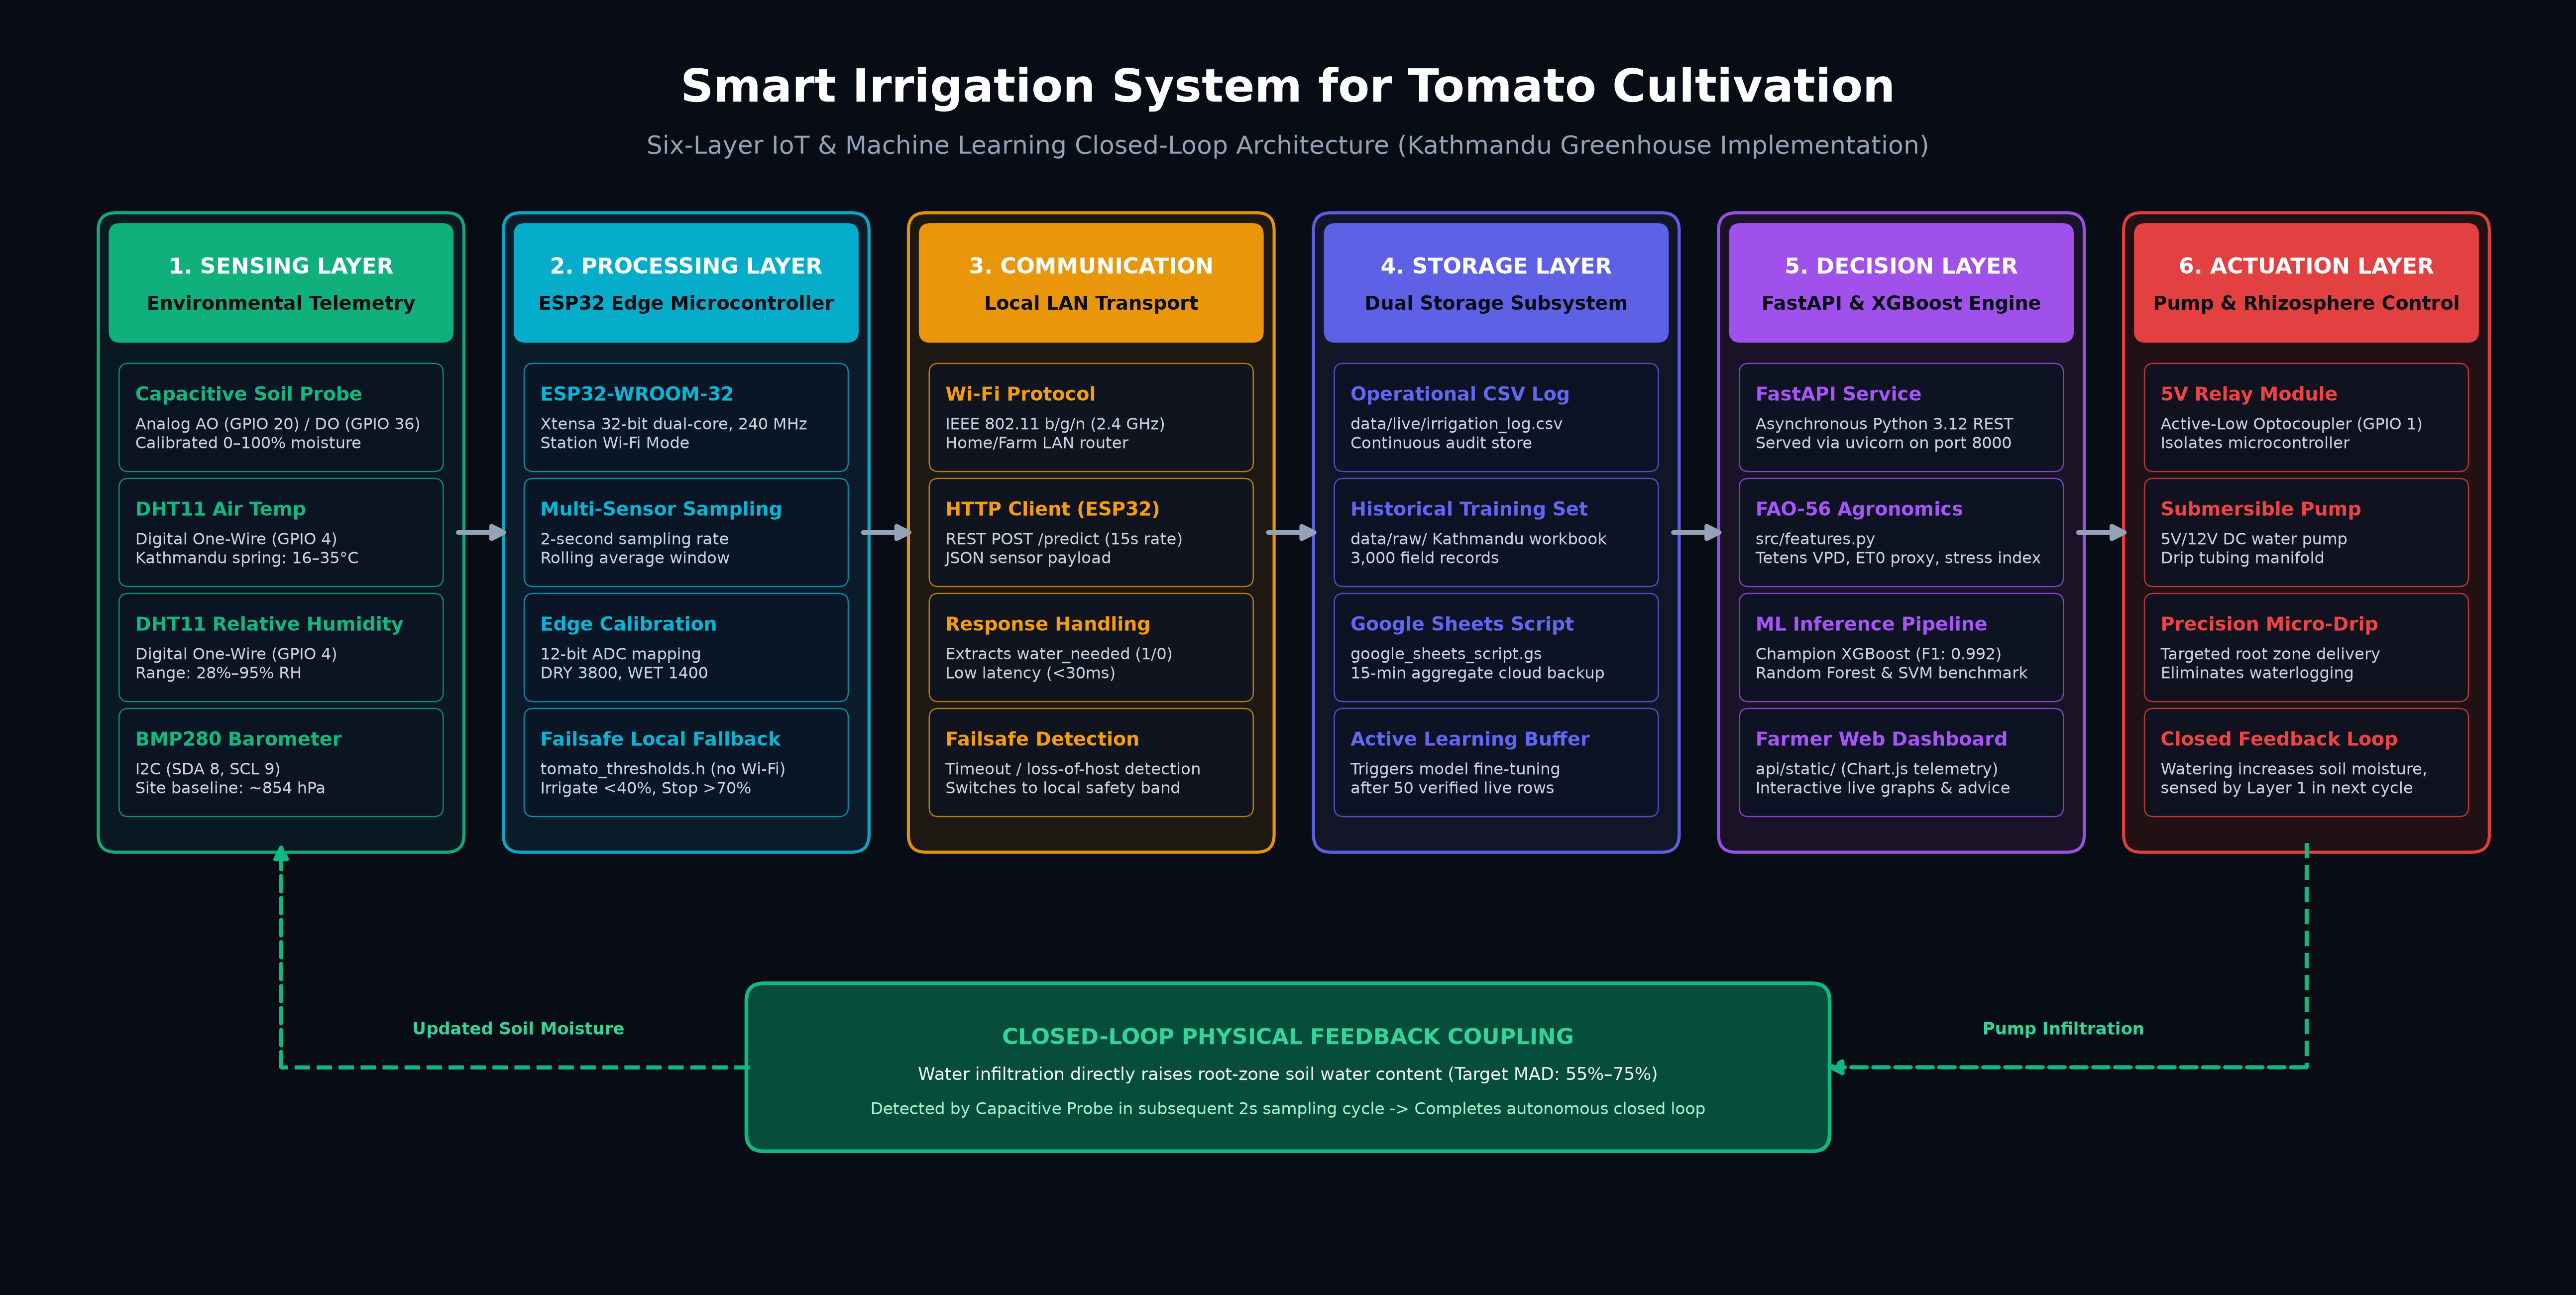
\includegraphics[width=0.98\textwidth]{Final_Year_Project_System_Design.png}
  \caption{Main system architecture of the smart irrigation artefact.}
  \label{fig:architecture}
\end{figure}

\begin{figure}[H]
  \centering
  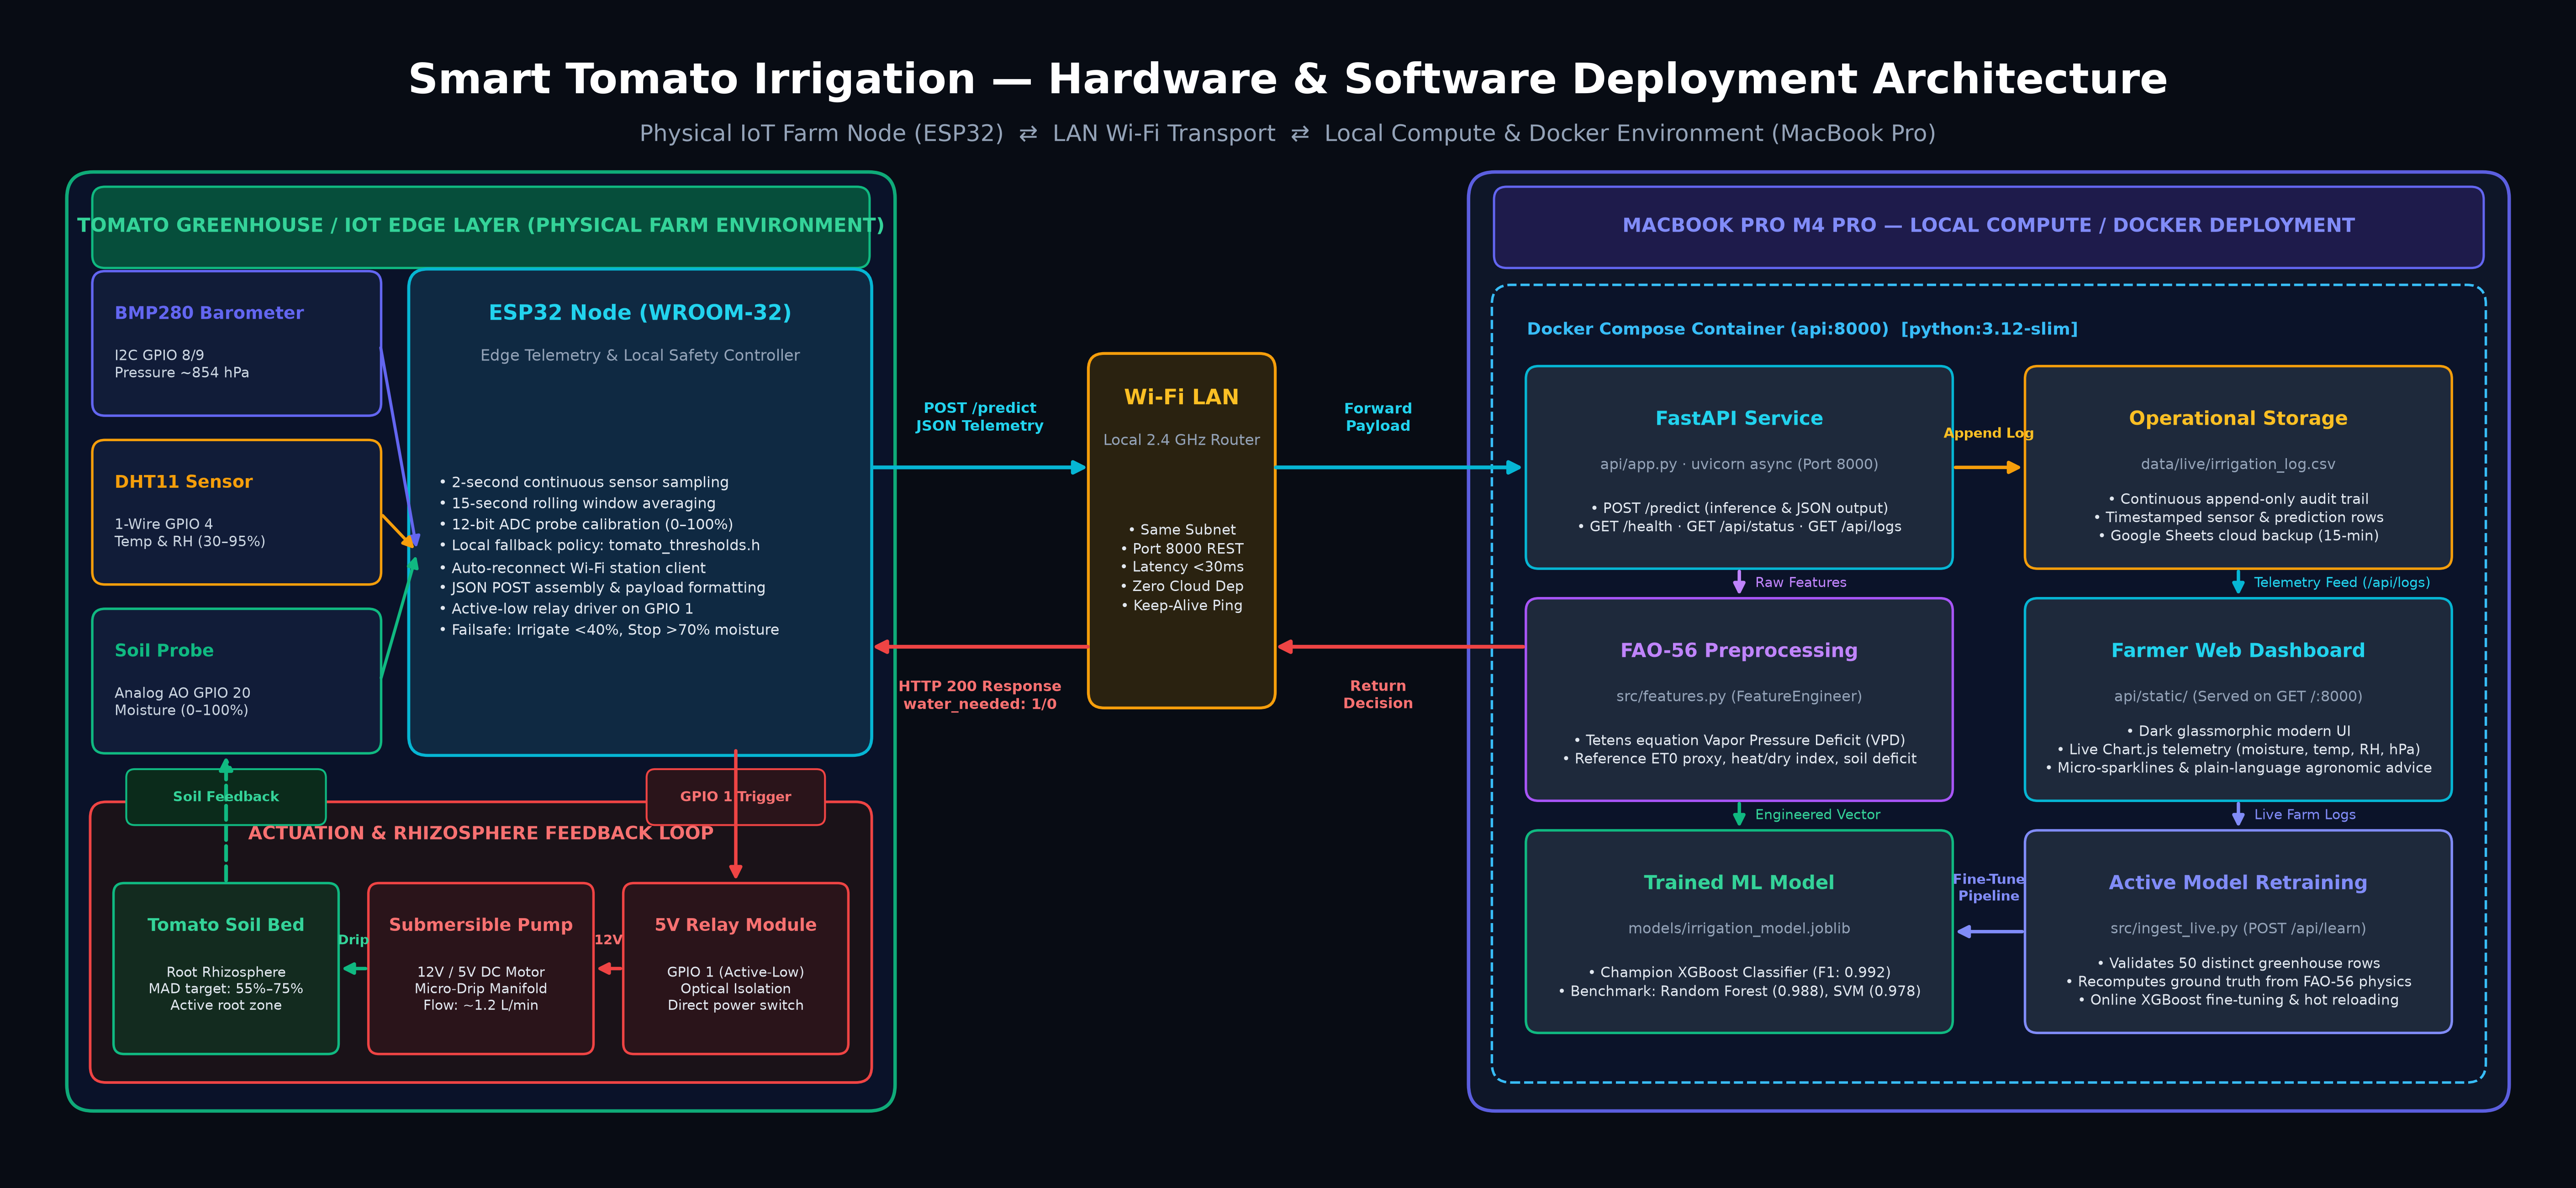
\includegraphics[width=0.98\textwidth]{deployment-architecture.png}
  \caption{Local deployment architecture (greenhouse node, Wi-Fi, FastAPI and XGBoost on the host computer).}
  \label{fig:deployment}
\end{figure}

\section{Implementation}
\label{sec:implementation}

\subsection{Construction of the Artefact}
\label{sec:construction}

Construction followed the six layers rather than a single ``write the model then add hardware'' sequence. Figure~\ref{fig:hardware} is the wiring; Figure~\ref{fig:serial} is a typical Serial log; Figure~\ref{fig:datacollect} is one \texttt{/predict} exchange. The relay (Figure~\ref{fig:relay}), dashboard (Figure~\ref{fig:dashboard}) and assembled prototype (Figure~\ref{fig:prototype}) are shown after the validation plots so that figure numbers run 1--17 in order.

\drawiofigure{fig04_physical_iot_hardware}{0.95\textwidth}{Physical IoT hardware and GPIO map.}{fig:hardware}

\drawiofigure{fig05_esp32_sensor_readings}{0.95\textwidth}{ESP32 sensor readings as shown on the Serial Monitor.}{fig:serial}

\drawiofigure{fig06_data_collection_example}{0.95\textwidth}{Data collection example: \texttt{POST /predict} body, response, and CSV log row.}{fig:datacollect}

\textbf{Data and labels.} The workbook was mapped from raw ADC-like soil values to 0--100\% moisture, pressure was checked against Kathmandu, and FAO-56 features were added. Exploratory plots showed the old pump tracking soil only, the tomato rule watering earlier in heat, and 92.2\% agreement between pump and tomato labels (207 extra ``water now'' decisions in heat; 26 holds where the tomato rule refused water). Dry soil (0--30\%) is always irrigated; wet soil (75--100\%) never is. The 55--75\% band is where climate features matter. Those findings justified the label change before any classifier was fit. Class balance on the tomato label is not extreme (350 irrigate vs 250 no-irrigate on the 600-row test split), so accuracy is not a misleading headline metric; F1 and recall are still reported because missing an irrigate decision dries the crop.

\textbf{Model training.} A stratified 80/20 split produced 600 test rows. XGBoost, Random Forest, and RBF SVM were trained with the feature transformer inside the pipeline so that production inference cannot forget VPD. Hyper-parameters stayed close to library defaults with a modest tree depth; the goal was a fair three-way comparison, not a Kaggle-style search. XGBoost won on F1 and recall and was written to \texttt{models/irrigation\_model.joblib}. A known pitfall was avoided: fitting the historical pump column yields near-perfect accuracy because that column \emph{is} a soil switch; it would not measure tomato-aware control. All reported scores use the FAO-56 \texttt{irrigate} label. Feature importance on the fitted booster concentrates on soil moisture and the FAO-derived deficit and VPD terms, which matches the agronomic story rather than an accidental correlation with pressure.

\textbf{API and dashboard.} FastAPI exposes \texttt{/health}, \texttt{/predict}, \texttt{/api/status}, \texttt{/api/logs}, and \texttt{/api/learn}. The predict body accepts the ESP32 field names (\texttt{temperature}, \texttt{humidity}, \texttt{soilMoisture}, \texttt{pressure}). A zero or missing pressure is replaced with 854.27~hPa. The response includes \texttt{water\_needed}, a probability, relay language, and one or two reasons (``The soil is too dry for tomato roots.''). Docker Compose is the supported deployment so that the ESP32 always talks to the same port. The dashboard refreshes every 3~s, shows a live pill if a reading arrived in the last 90~s, and stays on ``Waiting for sensors\ldots'' until a live post arrives. That empty state was important: it stops the farmer from thinking yesterday's row is today's soil.

\textbf{Firmware.} Sensor drivers were split into \texttt{aht10.cpp}, \texttt{bmp280.cpp}, and \texttt{soil\_moisture.cpp} but remain in one sketch directory. An earlier firmware called \texttt{ESP.restart()} after a Google Sheets upload, which tore down the control loop. That restart was removed so that Sheets is optional and the pump loop continues. Wi-Fi credentials stay in local firmware and are not committed. If FastAPI is unreachable, \texttt{updateTomatoRelay} still waters below 40\% and stops above 70\%, which is a conservative band inside the FAO range rather than a random guess.

\textbf{Live learning path.} At least 50 distinct greenhouse rows are required before \texttt{POST /api/learn} will merge and retrain. Labels are recomputed from sensors, not copied from \texttt{water\_needed}. The API reloads the joblib file when its modification time changes, so a grower does not have to restart Docker to pick up a new model.

Challenges included (i)~choosing HTTP and a local host instead of the interim MQTT/AWS stack, (ii)~refusing LSTM once EDA showed no timestamps, (iii)~keeping training and serving transformers identical, and (iv)~discovering that an uncalibrated soil probe reports 0\% even when air sensors are healthy. The last point is treated as a field-calibration task, not as a silent software failure. A fifth challenge was not to over-fit the story to the leaderboard: F1 near 1.0 on a rule-generated label is evidence that the pipeline learned the rule, which is necessary for serving, not evidence that tomato yield improved.

The implemented artefact meets the problem statement: irrigation is no longer a calendar. It answers the research questions with a working node, a measured F1, and a water-saving figure, while leaving season-length uptime open.

\subsection{Validation and Testing}
\label{sec:validation}

Validation used the held-out Kathmandu split, the objective scorer \texttt{src.evaluate\_objectives}, API tests, and the live CSV (2{,}729 rows from 1~September to 13~September 2026 in the scored extract).

\begin{table}[H]
\centering
\caption{Held-out test performance (600 rows) on the FAO-56 tomato label.}
\label{tab:leaderboard}
\begin{tabular}{lccccc}
\toprule
Model & Accuracy & Precision & Recall & F1 & ROC-AUC \\
\midrule
XGBoost (production) & 0.992 & 0.989 & 0.997 & \textbf{0.993} & 1.000 \\
Random Forest & 0.988 & 0.994 & 0.986 & 0.990 & 1.000 \\
RBF SVM & 0.985 & 0.989 & 0.986 & 0.987 & 0.999 \\
Soil $<$ 55\% cutoff & 0.923 & 0.987 & 0.880 & 0.931 & 0.939 \\
\bottomrule
\end{tabular}
\end{table}

Five-fold cross-validation F1 for XGBoost is $0.993 \pm 0.004$. Probability RMSE versus the 0/1 label is about 0.012. All three learned models beat the soil cutoff because they use VPD and heat as well as moisture (Figure~\ref{fig:mlcompare}).

\begin{figure}[H]
  \centering
  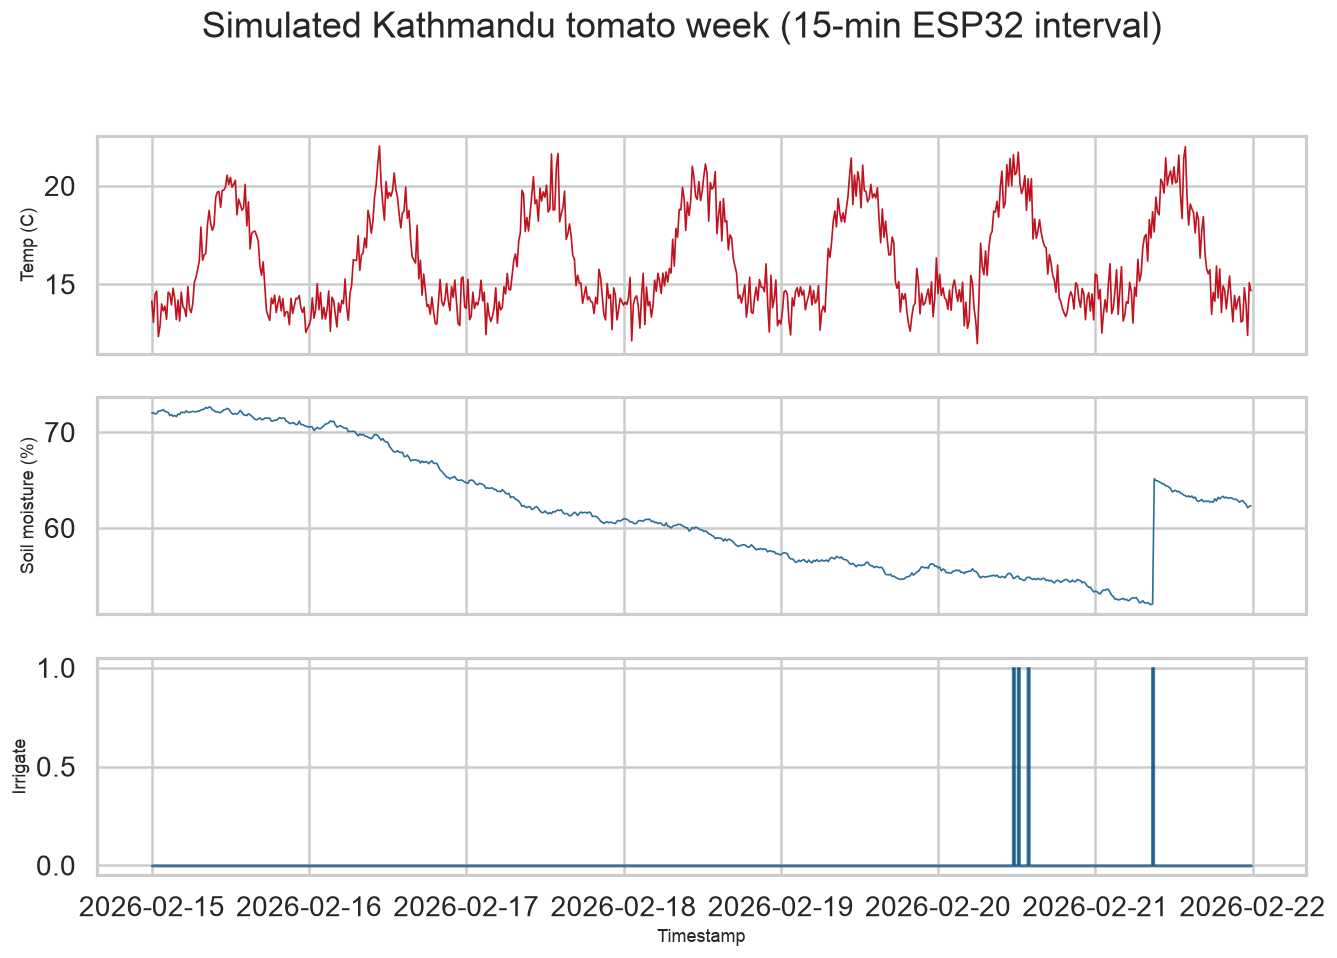
\includegraphics[width=0.92\textwidth]{07_season_week_timeseries.png}
  \caption{Sensor readings over time (FAO-56 simulated Kathmandu season used only for EDA).}
  \label{fig:timeseries}
\end{figure}

\begin{figure}[H]
  \centering
  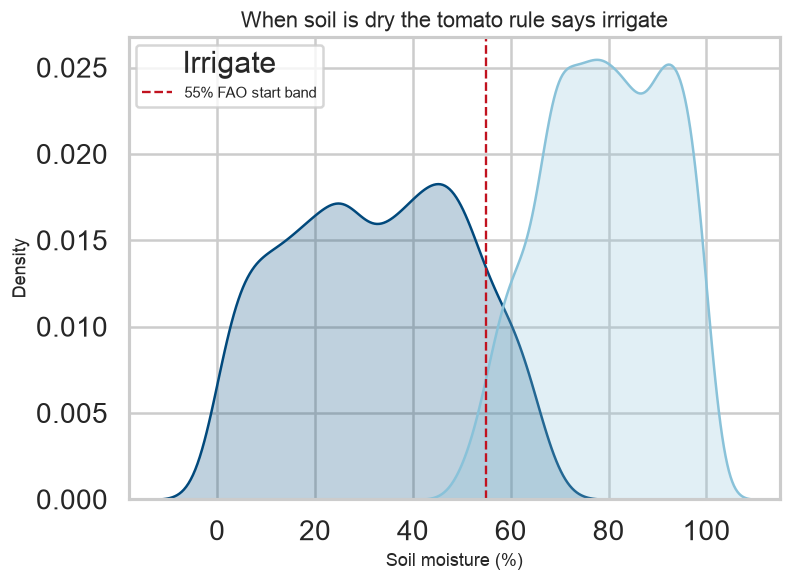
\includegraphics[width=0.88\textwidth]{09_soil_moisture_kde.png}
  \caption{Soil moisture distribution on the labelled training set.}
  \label{fig:soildist}
\end{figure}

\begin{figure}[H]
  \centering
  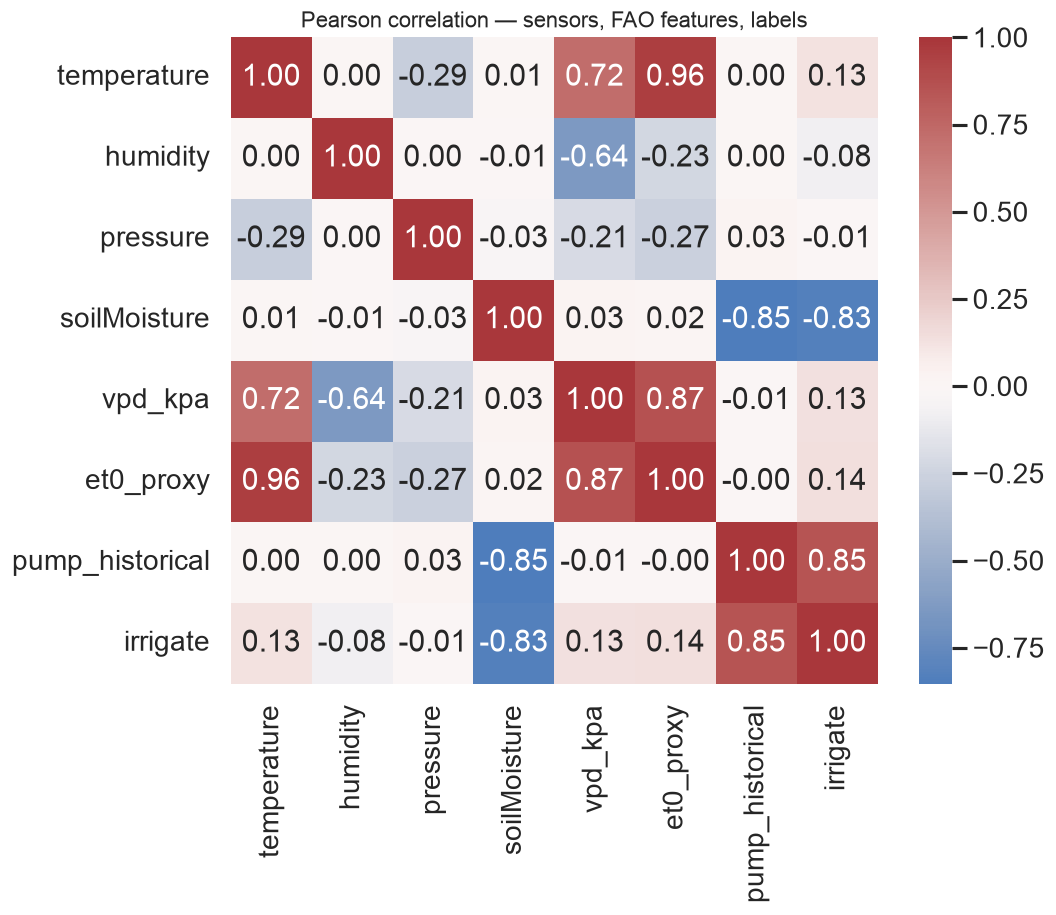
\includegraphics[width=0.82\textwidth]{03_correlation_heatmap.png}
  \caption{Correlation heatmap of the Kathmandu sensor and pump columns.}
  \label{fig:corr}
\end{figure}

\begin{figure}[H]
  \centering
  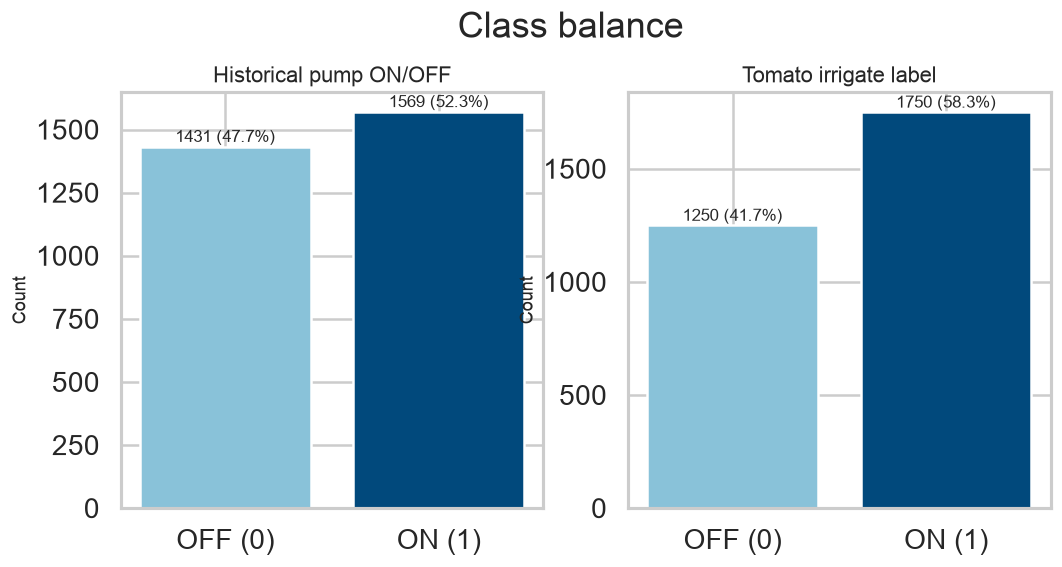
\includegraphics[width=0.82\textwidth]{06_class_balance.png}
  \caption{Water-needed (irrigate / wait) class distribution.}
  \label{fig:waterdist}
\end{figure}

\begin{figure}[H]
  \centering
  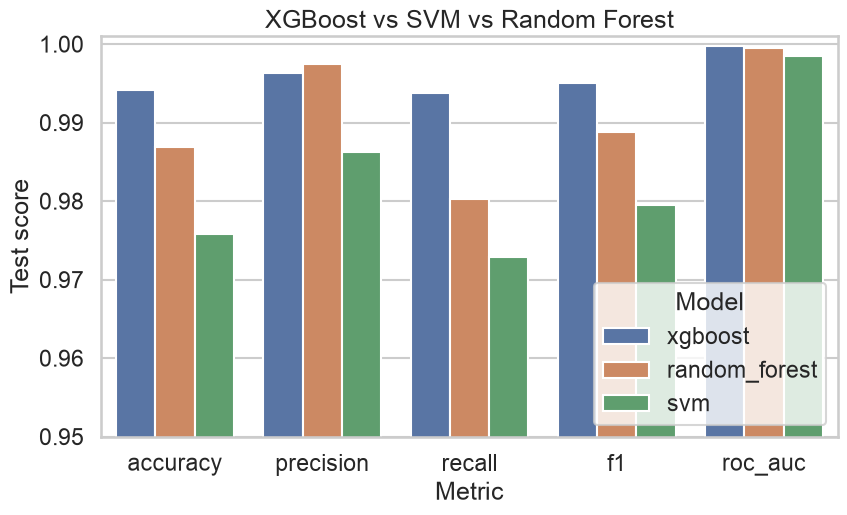
\includegraphics[width=0.88\textwidth]{14_model_comparison.png}
  \caption{ML model comparison on the held-out tomato-irrigation task.}
  \label{fig:mlcompare}
\end{figure}

\begin{figure}[H]
  \centering
  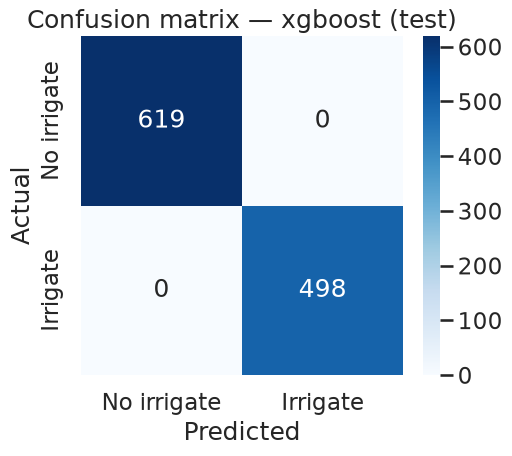
\includegraphics[width=0.72\textwidth]{10_confusion_matrix.png}
  \caption{Confusion matrix for the production XGBoost model (600-row test split).}
  \label{fig:cm}
\end{figure}

\begin{figure}[H]
  \centering
  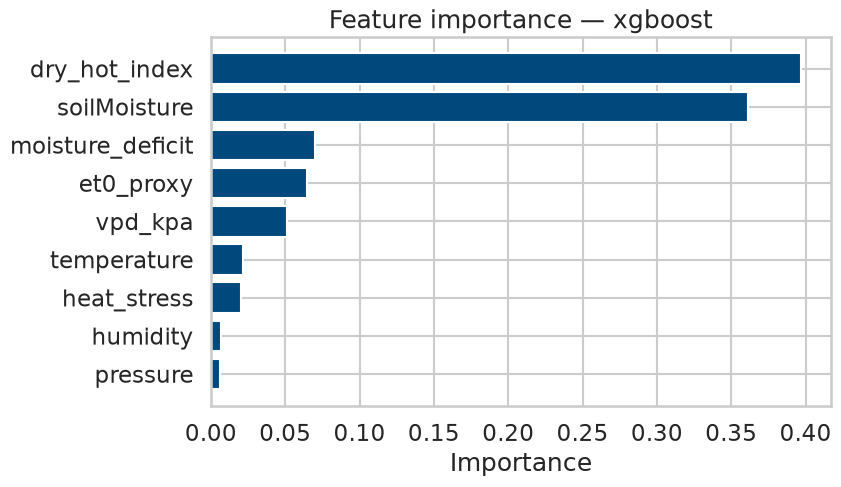
\includegraphics[width=0.82\textwidth]{12_feature_importance.png}
  \caption{XGBoost feature importance. Soil moisture and FAO-56 deficit/VPD terms dominate.}
  \label{fig:importance}
\end{figure}

Objective-level results on the scored snapshot:

\begin{itemize}[leftmargin=1.4cm]
  \item \textbf{O1 Sensing (partial).} Live rows contain temperature, humidity, and soil moisture from \texttt{device\_id=esp32-irrigation}. Air sensors are readable on 99.96\% of rows. About 99.9\% of live soil values are 0\%, so the ADC scale still needs \texttt{DRY\_SOIL}/\texttt{WET\_SOIL} calibration from Serial raw counts, or the probe is not in the root zone.
  \item \textbf{O2 Model (met).} Held-out F1 $0.993 \ge 0.90$. XGBoost, not LSTM.
  \item \textbf{O3 Water (met).} Model ON-fraction $0.583$ versus calendar $1.0$ $\Rightarrow$ 41.7\% saving. Wet soil ($\ge 75$\%) is never irrigated on 25.7\% of rows---water a timetable would waste. The FAO rule irrigates slightly more often than the old pump ($0.583$ vs $0.523$) because of heat; that is crop need, not calendar waste.
  \item \textbf{O4 Delivery (met).} Relay matches \texttt{water\_needed} on 100\% of live rows. One probe and one relay equal one tomato bed. Firmware timeout 8~s $<$ 10~s.
  \item \textbf{O5 Reliability (partial).} Median gap 16~s (target 15~s) while the host is up. Uptime versus a continuous 15~s schedule over the whole log span is about 4\%, because of long gaps (computer asleep, Wi-Fi, older restarting firmware). RH~$\ge 70$ is a usable wet proxy (1{,}308 rows); RH~$\le 50$ is almost absent in this window (1 row), so a true dry season is not yet in the log.
\end{itemize}

Pytest covers health and predict contracts. The combination of leaderboard, live agreement, and the objective JSON is the evidence that the artefact functions as specified---with the soil-calibration and host-uptime gaps named rather than hidden.

\begin{table}[H]
\centering
\caption{Interim evaluation metrics M1--M5 mapped to what this artefact reports.}
\label{tab:metrics}
\begin{tabularx}{\textwidth}{l l X}
\toprule
\textbf{Metric} & \textbf{Result} & \textbf{Notes} \\
\midrule
M1 accuracy & F1 $0.993$; prob.\ RMSE $0.012$ & LSTM RMSE not used; classifier matches the pump \\
M2 water saving & $41.7\%$ vs calendar & Always-on baseline; not a flow meter \\
M3 uptime & $\approx 4\%$ vs 15~s grid & Median gap 16~s while the host is awake \\
M4 latency & 8~s HTTP timeout & Under the 10~s target; one zone \\
M5 wet/dry & RH proxy only & 1{,}308 wet-leaning rows; almost no dry-season air \\
\bottomrule
\end{tabularx}
\end{table}

Paired $t$-tests on daily litres, promised in the interim evaluation plan, were not run: the workbook has no dates, and the live log has no flow sensor. Reporting a $p$-value on ON/OFF fractions would have been theatre. Descriptive rates and the leaderboard are the honest statistics.

\section{Critical Evaluation}
\label{sec:evaluation}

The farmer-facing result of that loop is the dashboard (Figure~\ref{fig:dashboard}), the relay/pump wiring (Figure~\ref{fig:relay}), and the assembled prototype (Figure~\ref{fig:prototype}). Export the matching draw.io files, or replace them with photographs and a screenshot.

\drawiofigure{fig14_web_dashboard}{0.95\textwidth}{Web dashboard at \texttt{GET /} (plain-language irrigation status).}{fig:dashboard}

\drawiofigure{fig15_pump_relay_setup}{0.95\textwidth}{Pump and relay setup driven from ESP32 GPIO~1.}{fig:relay}

\drawiofigure{fig16_final_working_prototype}{0.95\textwidth}{Final working prototype: sensors, node, host model, dashboard, and pump.}{fig:prototype}

The artefact is a working tomato irrigation controller: it senses, decides, and switches a pump, and it explains the decision to a person who is not a data scientist. In academic terms it sits between the ESP32 field systems of \citet{singha2025} and the neural forecast of \citet{meng2023}, but it does not copy either. Unlike Singha et al., the decision is tomato-specific FAO-56 plus a compared classifier, not a generic moisture trigger. Unlike Meng et al., there is no pretence that an LSTM was trained on data that cannot support one. That refusal is a contribution in a student project culture that often treats ``deep learning'' as mandatory.

\citet{singha2025} reported a 58\% water reduction and a 12\% yield gain on red amaranth. The 42\% ON-time reduction here is smaller and is not a yield trial, so it should not be advertised as matching their field outcome. It is still above the 30\% target inherited from that literature and from the interim report, and it is measured against a harsh calendar baseline (always on). Against the historical soil-only pump, ON-rate is slightly higher because FAO-56 waters more in heat. A reader who only compares to the old pump would wrongly conclude that the project ``uses more water''. The correct reading is: the project uses less water than a timetable and more crop-aware water than a soil switch.

Relative to a soil-only pump, the tomato label changes 7.8\% of decisions, concentrated in heat. Relative to a calendar, more than two-fifths of ON-time is dropped, including every waterlogged row. Those are the distinct advantages. The novel engineering piece is the closed loop on a local computer: joblib serving, CSV logging, live retrain that cannot poison itself, and firmware that keeps watering if the API dies. That is more modest than a cloud AIoT platform \citep{li2022}, and more deployable for the intended user. It is also more inspectable than a TFLite blob on a microcontroller: a supervisor can open the leaderboard CSV and the FAO-56 transformer and disagree with a threshold, which is how agronomy should meet software.

Significance is bounded. Held-out F1 near 1.0 is expected when labels are a smooth function of the same features the model sees; it does not prove that tomato yield rose in a randomised field trial. Water saving is ON-time, not litres through a flow meter. Spatial distribution is one bed, not a farm. Uptime is not yet 95\%. Live soil moisture is not yet a valid input. Those bounds are discussed in Section~\ref{sec:limitations}; they do not cancel the result that the loop works and that the classifier beats the obvious baseline. They do mean the strongest claims this report can make are about software-in-the-loop behaviour and held-out reconstruction of an FAO rule, not about a completed agronomic season.

% Word template numbering: section 7 then 7.2
\setcounter{subsection}{1}
\subsection{Impact}
\label{sec:impact}

For a Nepalese smallholder or a Kathmandu-valley tomato tunnel, the practical impact is a pump that can stay off when soil is wet and still run when air is hot and dry, without a subscription. Labour impact is smaller but real: the grower checks a sentence on a phone or laptop instead of guessing from the surface of the soil. For the local industry of student and NGO ``smart farm'' kits, the impact is a pattern that does not outsource control to AWS and that documents why LSTM was dropped. For academic discussion, the impact is a case where the right model family (tabular boosting) beat the fashionable one (LSTM) because of the data.

Societal value is water and labour: less standing water, fewer needless pump-hours, a dashboard an older grower can read \citep{zitan2021,upadhyay2015}. Environmental value is the 42\% ON-time cut versus a calendar on the historical set, in a country where dry-season water is already contested \citep{mool2001,kunwar2024}. There is also a negative impact to be honest about: an uncalibrated probe that always reads 0\% will ask the model to water as if the bed were dry. Until calibration, the local 40--70\% fallback and a farmer who can look at the plants remain the safety layer. The impact is potential until the soil probe is calibrated and the host stays awake for a season; it is not hypothetical in software, because the relay already follows the model on every live row that was logged.

\section{Conclusion}
\label{sec:conclusion}

The project started from a simple observation: Nepal's smallholders water by habit while global agriculture consumes most of the world's freshwater. The interim report proposed ESP32 sensing, an LSTM, MQTT to AWS, and solar power. The final artefact keeps the sensing and the water-saving ambition, and changes the decision and hosting layers to match the data and the pump. A six-layer loop now runs from a tomato bed to XGBoost on a local computer and back to a relay. Held-out F1 is 0.993; calendar ON-time falls by about 42\%; live actuation agrees with the API on every logged row. Objectives 2, 3, and 4 are met. Objectives 1 and 5 are partially met, limited by soil-probe calibration and host uptime. The aim---a working, evaluable, low-cost prototype---is achieved, with those two field tasks left explicit rather than claimed as finished.

\subsection{Limitations}
\label{sec:limitations}

\textbf{Labelling is a rule, not yield.} The FAO-56 tomato function is better agronomy than the historical pump, but it is still a heuristic. No fruit weight, Brix, or disease scores were collected, so ``better irrigation'' is not yet ``better crop''. Impact on the project: high F1 can coexist with a wrong rule. Mitigation: keep the rule documented and replaceable; do not treat XGBoost as an oracle.

\textbf{No timestamps on Phase~1 logs.} Stratified split can leak if rows from the same hour sit in both sides. Mitigation: report that limitation; use the live CSV, which is timestamped, for reliability rather than for the leaderboard.

\textbf{Live soil moisture is not yet trustworthy.} Nearly all live soil values are 0\%. Air sensors work, so the node is alive; the ADC mapping or probe placement is not. Mitigation: calibrate \texttt{DRY\_SOIL}/\texttt{WET\_SOIL} from Serial raw counts in the actual bed; until then, do not claim live soil-aware control.

\textbf{Uptime is host-bound.} A laptop that sleeps cannot meet a 95\% 15-second schedule. Old firmware that rebooted after Sheets made this worse. Mitigation: removed the restart; remaining fix is an always-on host (small PC or Raspberry Pi) rather than a student Mac.

\textbf{One zone, one season window.} Spatial Objective~4 is met only for one bed. Wet/dry Objective~5 uses RH bands, not two agricultural seasons. Mitigation: stated in the scope; a second node and a longer log are future work.

\textbf{Water saving is ON-time, not volume.} Without a flow meter, litres are inferred. Mitigation: treat 41.7\% as an upper-bound saving relative to always-on, not as a billed cubic-metre figure.

\textbf{No farmer trial.} Adoption insights from \citet{zitan2021} informed the dashboard wording but were not re-tested with Nepalese growers. Mitigation: qualitative interviews are listed under future work, not under results.

\subsection*{Future Work}
\addcontentsline{toc}{subsection}{Future Work}
\label{sec:future}

Concrete next steps follow the limitations. First, calibrate the soil probe in situ and confirm that live moisture spans dry-to-wet during a watering cycle. Second, move FastAPI to a small always-on host so that M3 uptime can be re-measured against 95\%. Third, add a cheap flow sensor so M2 becomes litres, not relay hours. Fourth, if a timestamped season log is collected, revisit a short-horizon sequence model as an \emph{addition} to XGBoost (tomorrow's ET0), not as a replacement for the 15-second relay bit. Fifth, replicate on a second bed to test spatial distribution. Sixth, run a small consent-based interview study with tomato growers on dashboard wording. Seventh, add the solar MPPT path of \citet{sohan2022} if the node leaves mains power. None of these steps requires discarding the current pipeline.

\newpage
% NOTE: verify conference entries in references.bib before submission.
\bibliography{references}

\appendix
\renewcommand{\thesection}{\Alph{section}}
\renewcommand{\thesubsection}{\Alph{section}.\arabic{subsection}}
\titleformat{\section}{\normalfont\Large\bfseries}{Appendix \thesection}{0.8em}{}

\section{Project Timeline}
\label{app:timeline}

The interim plan was 30 weeks in six phases. Table~\ref{tab:timeline} restates that schedule and records what was actually delivered by the final report.

\begin{table}[H]
\centering
\caption{Project timeline against the 30-week interim plan.}
\label{tab:timeline}
\begin{tabularx}{\textwidth}{l l X}
\toprule
\textbf{Weeks} & \textbf{Phase} & \textbf{Status at final report} \\
\midrule
1--4 & Literature, FAO-56 reading, hardware list & Complete (Section~\ref{sec:lit}) \\
5--10 & Hardware prototype, sensor bring-up & ESP32 + DHT11 + soil + BMP280 + relay working \\
11--14 & Interim report (week 14) & Submitted 15 April 2026; LSTM plan later revised \\
15--20 & Integration: API, model, firmware loop & FastAPI, XGBoost joblib, \texttt{/predict} closed loop \\
21--26 & Live log, evaluation, calibration & Live CSV and objective scores; soil ADC still to calibrate \\
27--30 & Final report and freeze & This document \\
\bottomrule
\end{tabularx}
\end{table}

\begin{figure}[H]
\centering
\begin{ganttchart}[
    hgrid,
    vgrid,
    x unit=0.31cm,
    y unit chart=0.52cm,
    title/.append style={fill=black!8},
    bar/.append style={fill=teal!35, draw=teal!70!black},
    milestone/.append style={fill=orange, draw=orange!70!black},
    bar height=0.45,
    milestone height=0.35,
]{1}{30}
  \gantttitle{Academic year (weeks 1--30)}{30} \\
  \gantttitlelist{1,...,30}{1} \\
  \ganttbar{Literature and FAO-56}{1}{4} \\
  \ganttbar{Hardware prototype}{5}{10} \\
  \ganttmilestone{Interim report}{14} \\
  \ganttbar{API, XGBoost, firmware loop}{15}{20} \\
  \ganttbar{Live log and evaluation}{21}{26} \\
  \ganttmilestone{Final report}{30}
\end{ganttchart}
\caption{Gantt chart of the 30-week project (Appendix~A).}
\label{fig:gantt}
\end{figure}

\section{Feasibility, Risks, and Ethical Aspects}
\label{app:feasibility}

This appendix revises the interim feasibility, risk, and ethics discussion now that the artefact exists.

\subsection{Revised Feasibility}
\label{app:feas}

The project was feasible on student time and budget. ESP32, DHT11, BMP280, and a capacitive probe are cheap and documented. Python, XGBoost, and FastAPI are free. No AWS IoT Core bill was required. The Kathmandu workbook removed the interim risk of having no Phase~1 data. Skills in embedded C++ and Python were sufficient; the main learning was FAO-56 feature design and refusing a poorly matched LSTM. Remaining feasibility risk is operational (keep the host awake, calibrate soil), not conceptual.

\subsection{Updated Risk Analysis and Mitigation}
\label{app:risk}

\begin{table}[H]
\centering
\caption{Risk assessment and mitigation (updated after implementation).}
\label{tab:risks}
\begin{tabularx}{\textwidth}{>{\raggedright\arraybackslash}p{3.6cm} c c X}
\toprule
\textbf{Potential risk} & \textbf{Likelihood} & \textbf{Impact} & \textbf{Mitigation strategy} \\
\midrule
Hardware delay or missing BMP280 & Medium & Medium & Order early; firmware substitutes 865~hPa; API substitutes 854.27~hPa. \\
Poor Wi-Fi or host asleep & High & High & HTTP timeout 8~s and local 40--70\% fallback; Docker on a machine that does not sleep; LoRa still a future field option. \\
Uncalibrated soil ADC (live 0\%) & High & High & Serial raw calibration of \texttt{DRY\_SOIL}/\texttt{WET\_SOIL}; do not retrain on live soil until the probe reads a range. \\
Insufficient or non-sequential training data & Medium & High & Use the 3{,}000 Kathmandu rows for Phase~1; do not force LSTM; merge live rows only with FAO labels. \\
Model/serving skew & Medium & High & Feature transformer inside the joblib pipeline; same code path in \texttt{src.train} and FastAPI. \\
Circular live learning & Medium & High & Refuse \texttt{/api/learn} until 50 rows; never use \texttt{water\_needed} as a label. \\
Firmware restart after Sheets & Medium & High & Removed \texttt{ESP.restart()} so the pump loop survives optional uploads. \\
\bottomrule
\end{tabularx}
\end{table}

\subsection{Revised Ethical Considerations}
\label{app:ethics}

No clinical data and no personally identifying farmer records are collected. Obligations still apply.

\textbf{Farmer involvement.} If the node is placed on land that is not the student's, written informed consent from the landowner is required before installation. No such off-site trial is claimed in this report.

\textbf{Data protection.} Live logs stay on the local computer as CSV. They are environmental measurements (temperature, humidity, soil, pressure, pump state), not names or phone numbers. They should not be published with Wi-Fi passwords or API URLs. Optional Google Sheets is an extra copy and should be disabled if the grower does not want data off-machine.

\textbf{Environmental responsibility.} The controller is intended to cut unnecessary pumping. It uses no agrochemicals. Solar power \citep{sohan2022} would further cut carbon if the node becomes off-grid; the present trial is mains-powered.

\textbf{Socio-economic impact.} Water and labour savings should accrue to the smallholder. The project does not automate farm labour out of existence; it removes a repetitive pump decision. Claims of livelihood impact are not made without a grower study.

\textbf{Integrity of claims.} Reporting XGBoost in place of the interim LSTM, and reporting soil-calibration and uptime failures, is treated as an ethical requirement: a final report that hid those facts would mislead a farmer who copied the kit.

\end{document}
